% Лекции Сергея Борисовича Стечкина
% Внесены исправления Ю.Н.Субботина и Н.И.Черныха, версия 30.06.2009
% Внесены исправления Н.И.Черныха, версия 29.07.2009
% Внесена грамматическая и ТеХ-правка М.Дейкаловой, версия 05.08.09

\chapter{Оценка остаточного члена интерполяции.\\
Многочлены Чебышева} %%{Лекция 2.}

\section{Оценка остаточного члена}

Пусть {$\{x_k\}^n_{k=0}$}~-- узлы интерполяции на $[a,b]$ и функция $f$ имеет непрерывную
${n+1}$ производную на $[a,b],$\ {$p_n(x,f)$~--
соответствующий} интерполяционный многочлен {Лагранжа} для $f,$\ $R_n(x,f)=f(x)-p_n(x,f)$~--
остаточный член интерполяции. Мы получили оценку
для $\|f(\cdot)-p_n(\cdot ,f)\|_C$ через наилучшее приближение
$E_n(f, \Cal P_n)_C$ (см. неравенство Лебега) и, значит, {(}так как $E_n(f,
\Cal P_n)_C \le \|f\|_C${)} через $\|f\|_C.$ Получили также оценку
$\|R_n(\cdot ,f) \|_C$ через максимум $f^{(n+1)}$ на отрезке, т.\,е. через
$\|f^{(n+1)}\|_C$ (см. {следствие из теоремы~\ref{t1-1})}. Следовательно, имеем оценки
\[
  \|f(\cdot )-p_n(\cdot ,f)\|_C \le
               \begin{cases}
                   \Cal K_0 \|f\|_C ,\\
                   \Cal K_{n+1} \|f^{(n+1)}\|_C ,
               \end{cases}
\]
где $\Cal K_0$ и $\Cal K_{n+1}$ -- соответствующие
независящие от функции константы. Попробуем оценить $\|R_n(\cdot ,f)\|_C$ через
{$\|f^{(m+1)}\|_C,$} т.\,е. получить оценки
\begin{equation}\label{lab1}
  \|R_n(\cdot ,f) \|_C \le  \Cal K_{m+1} \|f^{{(m+1)}}\|_C
\end{equation}
и для других $m,$ где $K_{m+1}=K_{m+1}(n)$ не зависят от $f.$
Если такие оценки справедливы, то, взяв функцию $f\in {\cal P}_m$,
у которой {$\|f^{(m+1)}(\cdot )\|_C=0$} получим, что $\|R_n(\cdot ,f)
\|_C=0,$ т.\,е. $f(x) \equiv p_n(x ,f)$ {~--} многочлен степени не выше
$n.$ Так что получаем {необходимое} ограничение на {числа $m,$}
для которых могут быть верны эти оценки: {$m \le n.$} Оценить $\|R_n(\cdot ,f) \|_C$
через нормы производных более высокого порядка нельзя,
так как из условия $f^{(m+1)}(x) \equiv 0,$~ $m > n,$ не следует, вообще
говоря, что $f(x) \equiv p_n(x ,f)$ (например, если $f$ есть
многочлен порядка {$m>n$}).

\begin{lemma}
Условие $m \le n$ является и достаточным условием для справедливости
оценки~$(\ref{lab1}).$
%$\|R_n(\cdot ,f) \|_C$
%через {$\|f^{(m+1)}(\cdot )\|_C.$}
\end{lemma}

\begin{proof}
Интерполяционная формула Лагранжа для $f$ имеет вид
\[
  p_n(x,f)=\sum\limits_{k=0}^n f(x_k) l_k(x).
\]
Используя тождество Коши $\sum\limits_{k=0}^n l_k(x) \equiv 1,$ получаем
$$
R_n(x,f)=f(x)-\sum\limits_{k=0}^nf(x_k)l_k(x)=\sum\limits_{k=0}^n \{f(x)-f(x_k) \} l_k(x).
$$
Запишем для $f(y)$ формулу Тейлора порядка $m$ в точке $x$ с остаточным
членом в интегральной форме
\[
  f(y)=f(x)+p(x,y)+\frac{1}{m!}\int_x^y (y-t)^m f^{(m+1)}(t)dt,
\]
где $f(x)+p(x,y)=q_x(y)$~-- многочлен Тейлора функции $f$ в точке $x.$ В частности,
\[
 f(x_k)=f(x)+q_x(x_k)+\frac{1}{m!}\int_x^{x_k} (x_k-t)^m f^{(m+1)}(t)dt,
\]
где
$$
q_x(x_k) = \sum\limits_{s=1}^m\frac{1}{s!}f^{(s)}(x)(x_k-x)^s
$$
($q_x(x_k)$~-- не многочлен по $x$).

Подставим $f(x_k)$ в выражение для $R_n(x,f),$ при этом учтем, что в
силу третьего тождества Коши \eqref{f1-1} при $m \le n$
$$
\sum\limits_{k=0}^n q_x(x_k)l_k(x)=\sum\limits_{{s=1}}^m{\frac{1}{s!}f^{(s)}(x)
 \sum\limits_{k=0}^n{(x_k-x)^s}l_k(x)}\equiv
0.
$$
{Получим}
\[
{  R_n(x,f)=-\frac{1}{m!} \sum\limits_{k=0}^n l_k(x)
                         \int_x^{x_k} (x_k-t)^m f^{(m+1)}(t)dt=
                         \int_a^b K_{n,m}(x,t,\{x_k\}) f^{(m+1)}(t)dt,}
\]
{Можно проверить, что ядро $K_{n,m}(x,t,\{x_k\})$} этого
выражения при каждом $x$ только при $m=n$ не {меняет знак при $t \in
[a,b]$} и только в этом случае можем,
{применив теорему о среднем,} записать
\[
  R_n(x,f)=f^{(n+1)}(\xi) \cdot A(x)\qquad {(\xi = \xi(x, f, K_{n,n})),}
\]
где $A(x)$ от $f$ не зависит. {Но во} всех {рассматриваемых} случаях {(т.\,е.
при $m \le n$)} получим оценку
\[
  |R_n(x,f)| \le \|f^{(m+1)}(\cdot )\|_C
        \int_a^b |K_{n,m}(x,t,\{x_k\})| dt,\qquad x \in [a,b],
\]
из которой следует требуемое неравенство~(\ref{lab1}).
\end{proof}

\section{Многочлены Чебышева}

Многочленами Чебышева $T_n(x)$ {называются функции}
$$
  T_n(x)=\cos (n\arccos x) \qquad (n=0,1,\dots ),\qquad  x \in [-1,1].
$$
Это, действительно, многочлены: положим $x= \cos \theta$,~ {$\theta \in [0, \pi],$} тогда
%\begin{multline*}
$$
\begin{aligned}
T_n(x) &=\cos (n \arccos x)= \cos n\theta = {\frac{1}{2}(e^{in\theta} +
e^{-in\theta})
=} \\
   &=\frac{1}{2}\{(\cos \theta +i \sin \theta)^n+(\cos \theta -i \sin \theta)^n\}.
\end{aligned}
$$
%\end{multline*}
{Следовательно, при $|x| \le 1$}
$$
T_n(x)=\frac{1}{2}\{(x +i \sqrt{1-x^2})^n+(x -i \sqrt{1-x^2})^n\}.
$$
Из последнего выражения видно, что мнимые части {здесь} уничтожаются, {а в}
{вещественной части радикалы отсутствуют}.

\begin{ex}
{Как многочлен, функция $T_n(x)$ определена при всех $x$. Найти} {для него
представление при $|x| > 1$, аналогичное последней формуле.}
\end{ex}

\section{Основные свойства многочленов Чебышева \\
(выражаемые равенствами)}

\vspace{-2mm}
{\bf 1. Рекуррентная формула}
\vspace{3mm}

При $n=0$ и $n=1$ имеем $T_0(x) \equiv 1,$ $T_1(x) \equiv x.$ Из тригонометрического тождества
\[
  \cos (n+1)\theta =2 \cos \theta \cos n \theta -\cos (n-1)\theta
  \qquad (x = \cos{\theta})
\]
следует {рекуррентная формула}
\[
  T_{n+1}(x)=2x T_n(x)-T_{n-1}(x) \qquad (n=1,2,\dots ).
\]
{Имеем также}
$$
 {T_n'(x)=n \sin ({n} \arccos{x})\cdot \frac{1}{\sqrt{1-x^2}} = \frac{n\sin
 n\theta}{\sin{\theta}}.}
$$

Из рекуррентной формулы следует, что коэффициент при старшей степени многочлена
{$T_n(x)$ при $n \ge 1$} равен $2^{n-1}$, так что
\[
  T_n(x)=\cos (n \arccos x) =2^{n-1} x^n+\cdots .
\]
Все нули этого многочлена $x_k=\cos \dfrac{2k-1}{2n}\pi$
$(k=1,2,\dots ,n)$ лежат в~$(-1,1).$ {Точками} экстремумов
на $[-1,1]$ являются {точки} $\widetilde x_k=\cos \dfrac{k
\pi}{n}$ {$(k=0,1,\dots ,n),$} $T_n(\widetilde x_k)=(-1)^k,$
причем при {$k\ne 0$} и {$k \ne n$} выполнено {условие
$T_n'(\widetilde x_k) = 0,$ а $T_n'(1)=n^2,$}\
{$T_n'(-1)=(-1)^{n-1}n^2$. С ростом $n$ нули и точки
экстремума уплотняются у концов} {отрезка $[-1,1]$} (сравним
рис.~\ref{r2-1} и \ref{r2-2}).

%%%%%%%%%%%%%%%%%%%%%%%%%%%%%%%%%%%%%%%%%%%%%%%%%%%%%%
%\hbox to 0.5cm {}{\special{em:graph pict7.pcx}}
%\vspace{6cm} \vspace{5mm} \noindent
%\begin{picture}(0,170)
% \put(0,160){\special{em: graph pict2-1.pcx}}
% \end{picture}

\begin{center}
\begin{picture}(290,100)
\includegraphics[width=0.95\textwidth]{pict02-1.eps}
\end{picture}
%\bigskip
\centerline{\normalsize Рис.~\theris}

\refstepcounter{ris}\label{r2-1}
\end{center}


%\vspace{-3mm}
{\bf 2. Производящая функция}
\vspace{3mm}

Если дана последовательность $\{A_n\},$ то {ее} производящей функцией называется
такая функция $F,$ коэффициенты Тейлора которой равны $A_n.$

Вычислим {$\sum\limits_{n = 0}^{\infty} \cos (n\theta )\ {t^n}.$}
Это действительная часть степенного ряда
\[
  \sum\limits_{{n=0}}^{\infty}\, \exp{(i n\theta)}\ t^n=\frac{1}{1-t\exp{(i \theta)}}
 { =\frac{1-t\exp(-i\theta)}{1-2{t}\cos{\theta}+t^2},}
\]
так что
\[
  \sum\limits_{{n=0}}^{\infty}\, \cos (n\theta )\ {t^n}=
                      \frac{1-t \cos \theta}{1-2t\cos \theta +t^2}
\]
и если $x=\cos \theta,$ то получаем производящую функцию {$F(t)$} для {последовательности}
многочленов Чебышева:
\[
  \sum\limits_{n=0}^{\infty} T_n(x)\,t^n=\frac{1-tx}{1-2tx+t^2}.
\]
{Заменим здесь $x$ на $-x$. Получим}
$$
{\sum\limits_{n=0}^\infty{T_n(-x)t^n} = \sum\limits_{n=0}^\infty{T_n(x)(-t)^n}}
$$
{и, следовательно, $T_n(-x)=(-1)^nT_n(x)$. Конечно, это
свойство можно вывести и из} {явного представления для
$T_n$.}

\ex Как растут {$|T_n(x)|$} в точках $|x|>1$ {с ростом $n$?}

\noindent {У к а з а н и е.\ \ Воспользоваться представлением}
$$
{T_n(x)=\frac{1}{2}\left \{(x +\sqrt{x^2-1})^n+(x -
\sqrt{x^2-1})^n \right\}, \qquad |x|>1.}
$$

\vspace{3mm}
{\bf 3. Дифференциальное уравнение}
\vspace{3mm}

Дифференциальное уравнение, которому удовлетворяют $T_n$:
\[
  (1-x^2)y''-xy'+n^2y=0\qquad (n=0,1,\dots ).
\]
\ex Проверить.

Будем искать {коэффициенты многочлена}
$$
{ T_n(x)=\sum\limits_{k=0}^n a_kx^{n-k}}
$$
{при $n\ge 2$, зная, что он} удовлетворяет этому уравнению. {Знаем также, что}
$a_0=2^{n-1}$ {и} $a_1=a_3=\cdots =0,$ {так как $T_n(-x)=(-1)^nT_n(x).$} Тогда,
подставив в дифференциальное уравнение, получим рекуррентное соотношение
\[
  a_{2k}=-\frac{(n-2k+2)(n-2k+1)}{4k(n-k)}a_{2k-2}.
\]
Следовательно,
\[
  a_{2k}=\frac{(-1)^k n(n-1)\cdots (n-2k+1)}{4^kk!(n-1)\cdots (n-k)}\,{a_0}=
  (-1^k)
  \frac{n}{n-k}C^k_{n-k}2^{n-2k-1}
\]
{и}
$$
  T_n(x)=\sum\limits_{k=0}^{[n/2]} a_{2k}x^{n-2k}.
$$

\begin{Remark}
Несмотря на то, что многочлены Чебышева ограничены единицей на $[-1,1],$ его
коэффициенты при больших $n$ очень большие.
\end{Remark}

\vspace{3mm}
{\bf 4. Ортогональность}
\vspace{3mm}

{Справедливы равенства}
\[
{\frac{2}{\pi}} \int_{-1}^1 \frac{T_n(x)T_m(x)}{\sqrt{1-x^2}}dx={\delta_{n,m}}.
\]

\begin{ex}
{Проверить, сделав замену $x=\cos{\theta}$~ $(0 \le \theta \le \pi)$.}
\end{ex}

\section{Экстремальные свойства многочленов Чебышева}

%\vspace{3mm}
{\bf 1. Первое экстремальное свойство}
\vspace{3mm}

Нормированный многочлен Чебышева $\widetilde T_n(x)=\dfrac{T_n(x)}{2^{n-1}}$ есть многочлен, наименее уклоняющийся от нуля на $[-1,1]$ среди
всех многочленов со старшим коэффициентом $1,$ т.\,е. имеет место {следующее утверждение.}

\begin{teo} \label{teo1extsvo}
Справедливы равенства
%{\it
%\begin{multline*}
$$
\inf_{p \in \Cal P_n,\ p =x^n+\dots} \|p(\cdot )\|_{C[-1,1]} =
            \|\widetilde T_n(\cdot )\|_{C[-1,1]}=\frac{1}{2^{n-1}}=
$$
$$
=\inf_{p \in \Cal P_{n-1}} \|x^n-p(x)\|_{C[-1,1]}= E_{n-1}(x^n)_{C[-1,1]},
$$
%\end{multline*}
где $$\widetilde T(x)=\dfrac{1}{2^{n-1}}T_n(x)=x^n+\dots$$ -- нормированный
многочлен Чебышева. Наилучшее приближение
$E_{n-1}(x^n)_{C[-1,1]}$ достигается на
многочлене $p(x)=x^n-\dfrac{1}{2^{n-1}}T_n(x)\in {\cal P}_n$ {и только на нем}.
\end{teo}

\begin{proof}
Основная идея доказательства заключается в подсчете числа нулей. Пусть есть многочлен
$p \in \Cal P_n$ %с той же нормировкой,
{со старшим коэффициентом, равным $1$,}
но {такой, что}
$$
  \|p(\cdot )\|_{C[-1,1]}  \le \|\widetilde T_n(\cdot )\|_{C[-1,1]}.
$$
Тогда на каждом отрезке, где {$T_n(x)$} изменяется от {$\pm 1$} до {$\mp 1,$ т.\,е. на }
{отрезках $[\widetilde x_k, \widetilde
x_{k+1}]\ (\widetilde x_k=\cos \dfrac{k\pi}{n}$, \
$k={0,1,}\ldots,n$)} разность {$r_{n-1}(x)=\widetilde T_n(x)-p(x)$} обращается в нуль
{(при этом мы учитываем, что если $r_{n-1}=0$ в общем конце двух} {таких отрезков,
то там $T'$ и $p'$ обращаются в нуль и, значит, это
двойной нуль} {разности $r_{n-1}(x)$, см.~рис.~\ref{r2-2}).} {Таким образом,}
степень многочлена $r_{n-1}$ не выше $n-1,$ {а число его
нулей с учетом кратности $\ge n.$} {Следовательно,} $r_{n-1} \equiv 0,$ {$p(x)
\equiv \widetilde T_n(x),$ откуда вытекают все утверждения
теоремы~\ref{teo1extsvo}.} %\pagebreak

%%%%%%%%%%%%%%%%%%%%%%%%%%%%%%%%%%%%%%%%%%%%%%%%%%%%%% %\hbox to 0.5cm {}{\special{em:graph pict8.pcx}} %\vspace{6cm} \vspace{5mm} \noindent
%\begin{picture}(0,210)
% \put(0,190){\special{em: graph pict2-2.pcx}}
% \end{picture}
% \refstepcounter{ris}\label{r2-2}
\begin{center}
\begin{picture}(320,130)
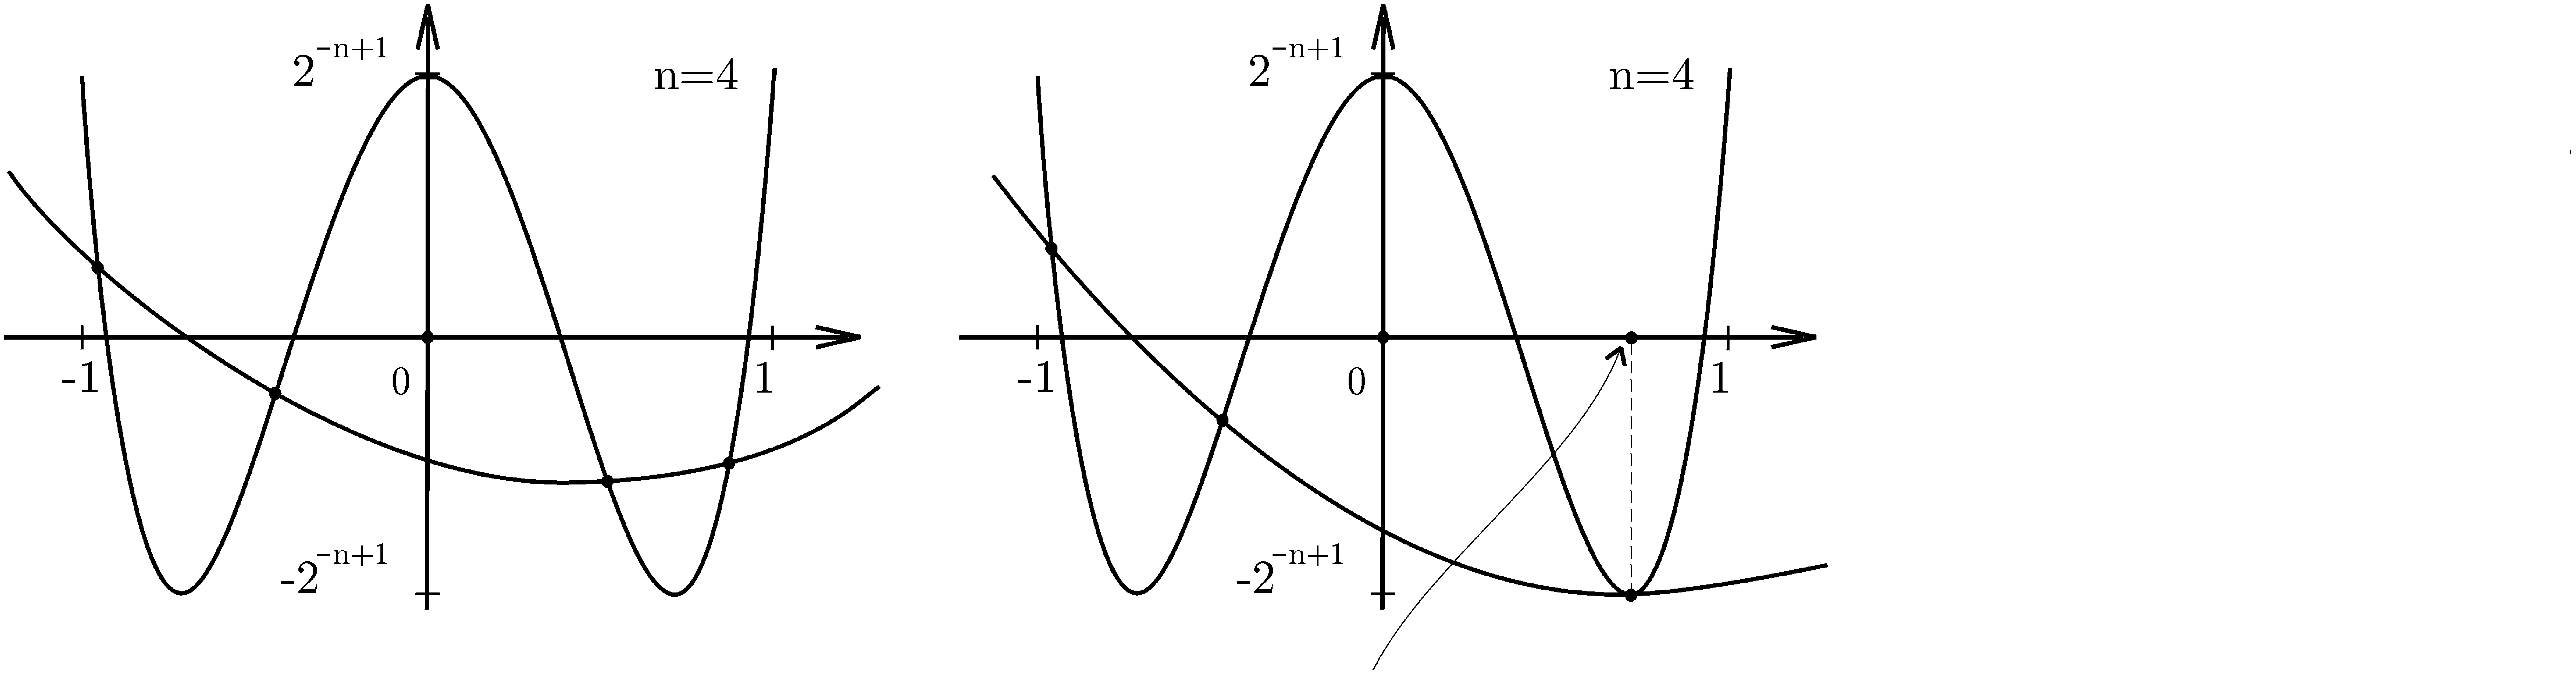
\includegraphics[width=0.99\textwidth]{pict02-2.eps}
\end{picture}
%\bigskip

\refstepcounter{ris}\label{r2-2}
\end{center}

%\centerline{Рис.~\theris}
 \hspace{9.5cm} {Двойной нуль}


 \centerline{\normalsize Рис.~\theris}
\end{proof}

\vspace{2mm}
{\bf 2. Второе экстремальное свойство}
\vspace{3mm}

\begin{lemma}
Пусть {$p \in \Cal P_n,$~ $|p(x)| \not\equiv |T_n(x)|\cdot \|p\|_{C[-1,1]},$} и пусть
$\xi \in \bR,$~ $|\xi |>1.$ Тогда
\[
{ |p(\xi )| < |T_n(\xi)|\cdot \|p(\cdot )\|_{C[-1,1]}.}
\]
{Равенство хотя бы в одной точке $\xi$ вне $[-1,1]$ здесь возможно, только если}
{$p(x)\equiv 0$ {или
$\dfrac{|p(x)|}{\|p\|_{C[-1,1]}}\equiv |T_n(x)|.$}}
\end{lemma}

Д о к а з а т е л ь с т в о\ \ от противного. {Предположим,} {что $\exists\ \xi
\not \in [-1,1]$ :} {$|p(\xi)|
\ge |T_n(\xi)|\cdot\|p\|_{C}$.} Разность
{$q(x)=\dfrac{p(x)}{\|p_n\|_{C[-1,1]}}-T_n(x)$} {-- нетривиальный} многочлен степени
{не выше} $n$ и не может иметь {больше $n$
нулей.} { Пусть для определенности $\xi<-1$,~ $\dfrac{p(\xi)}{\|p\|_{C}}
\ge T_n(\xi) > 0$ (т.\,е. $n$ -- четное, $p(\xi)>0$).}
{Считаем нули. Ясно, что на отрезке $[\xi,-1]$ найдется точка}
{$\xi_0,$ в которой $q(\xi_0)=0.$}

%%%%%%%%%%%%%%%%%%%%%%%%%%%%%%%%%%%%%%%%%%%%%%%%%%%%%%
%\hbox to 0.5cm {}{\special{em:graph pict9.pcx}} %\vspace{6cm} \vspace{5mm}
 %\bigskip
 %\begin{picture}(110,200)
 %\put(110,200){\special{em: graph pict2-3.pcx}}
 %\end{picture}
 %\refstepcounter{ris}\label{r2-3}

 %\centerline{Рис.~\theris}
 %\bigskip

 \begin{center}
\begin{picture}(160,128)
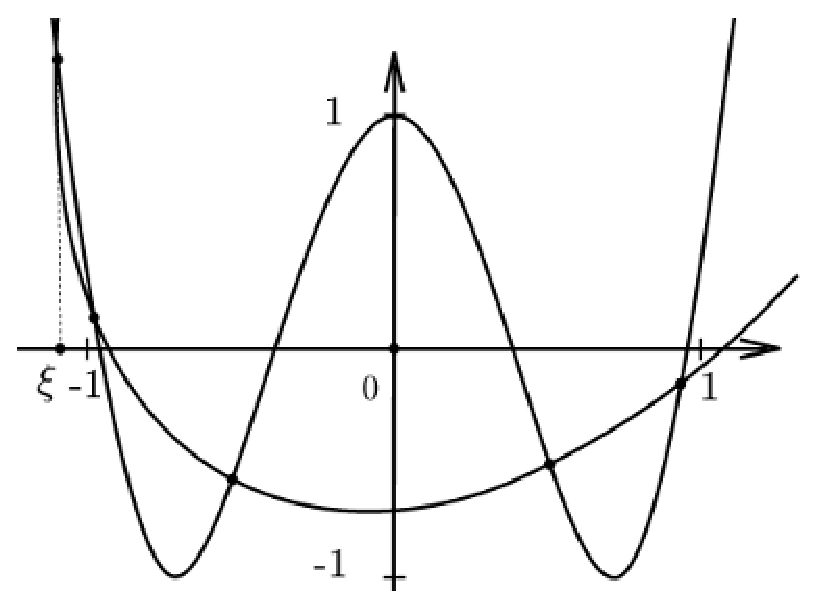
\includegraphics[width=0.34\textwidth]{pict02-3.eps}
\end{picture}
\vspace{5mm}
\refstepcounter{ris}\label{r2-3}
\end{center}

\centerline{\normalsize Рис.~\theris}


%%%%%%%%%%%%%%%%%%%%%%%%%%%%%%%%%%%%%%%%%%%%%%%%%%%%%%%%%% %\noindent \hskip3.0cm {рис. 9}

%\centerline{рис.9}


\noindent

{Далее, график полинома $y{(x)}=\dfrac{p(x)}{\|p\|_{C}}$ на отрезке
$[-1,1]$ не выходит за полосу $|y| \le 1.$ Поэтому, рассуждая как при
доказательстве теоремы~\ref{teo1extsvo}, получаем, что $q(x)$ имеет на
$[-1,1]\quad n$ нулей с учетом их кратности. Если к тому же $\xi_0 < -1$
{(см. рис.~\ref{r2-3})}, то получаем $q(x) \equiv 0$ на $\bR.$
Если же $\xi_0=-1$ и $q(x) \ne 0$ на промежутке $[\xi, -1),$ то рассуждать
нужно чуть потоньше. Во-первых, может оказаться, что $\xi_0=-1$~-- нуль
второго порядка~-- двойной корень $q.$ Ясно, что один из них не вошел в
число учтенных $n$ нулей на отрезке $[-1,1],$ так как из двойных нулей
были учтены только совпадающие с некоторыми из $\widetilde x_k=\cos
\dfrac{k\pi}{n}$~ $(k=1,2,\ldots,n-1).$}

{Вторая возможность~-- $q'(\xi_0) \ne 0$ {$(\xi_0=-1)$.}
Тогда $q(x)$ в
точке $\xi_0=-1$ меняет знак с $+$ на $-$, график $p(x)$ в
правой полуокрестности точки {$\xi_0$} окажется ниже
графика~$T_n.$ Следовательно в обоих случаях {на промежутке $[-1,\widetilde{x}_{n-1}]$}
{у полинома $q(x)$ будет не менее двух нулей,} общее число
нулей будет $\ge n+1.$ Значит, опять $q(x) \equiv 0$ на $\bR,$
что противоречит предположению.}

{Общий случай (без предположений $\xi < -1$ и $n$~-- четное) сводится к
рассматриваемому заменой $p$ и $T_n$ на $-p,\ -T_n$ и/или $T_n(x)$ на $T_n(-x)$. Лемма
доказана.}

%\end{proof}


{Таким образом, если $\|p_n\|_{C[-1,1]} \le 1,$~ $p_n \in \Cal P_n,$ и
$|\xi|>1,$ то $|p_n(\xi)| \le |T_n(\xi)|.$}

\ex {Доказать, что если $p \in \Cal P_n$ и}
$\|p(\cdot )\|_{C[-1,1]} \le 1,$ то $|p'(1)| \le T_n'(1)$ (для доказательства
опять считаем нули), {см. рис.~\ref{r2-4}}.

{Имея ввиду это свойство, $T_n$} называют многочленом сравнения.

%%%%%%%%%%%%%%%%%%%%%%%%%%%%%%%%%%%%%%%%%%%%%%%%%%%%%% %\hbox to 0.5cm {}{\special{em:graph pict10.pcx}} %\vspace{6cm} \vspace{5mm}
%\begin{picture}(100,170)
% \put(100,160){\special{em: graph pict2-4.pcx}}
% \end{picture}
% \refstepcounter{ris}\label{r2-4}

% \centerline{Рис.~\theris }
% \bigskip


 \bigskip
\begin{figure}[ht]
\begin{center}
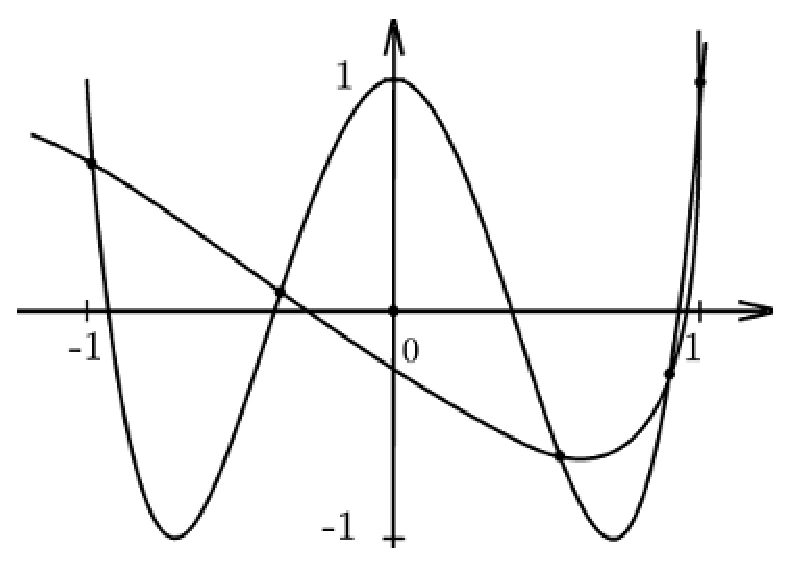
\includegraphics[width=0.35\textwidth]{pict02-4.eps}
\end{center}
 \bigskip
 \refstepcounter{ris}\label{r2-4}

 \centerline{Рис.~\theris}
 \bigskip
\end{figure}




\begin{Remark}
Из леммы~2.2 следует, что если $[-a,a] \supset [-1,1]$
 и $p_n \in \Cal P_n,$ то справедливо неравенство
\[
  \|p(\cdot )\|_{C[-a,a]} \le \|T_n(\cdot )\|_{C[-a,a]}\cdot \|p(\cdot )\|_{C[-1,1]},
\]
{где знак равенства возможен только при $p(x)\equiv 0$ или $p(x)\equiv\pm T_n(x)
\|p(\cdot )\|_{C[-1,1]}$.}
\end{Remark}
